\section{337 --- House Robber III}

\textbf{Medium}

The thief has found himself a new place for his thievery again. There is only one entrance to this area, called the \textit{root}. Besides the root, each house has one and only one parent house. After a tour, the smart thief realized that \textit{all houses in this place forms a binary tree}. It will automatically contact the police if two directly-linked houses were broken into on the same night.

Determine the maximum amount of money the thief can rob tonight without alerting the police.

\paragraph{Example 1:}
\begin{flushleft}


\textbf{Input}: \fcj{[3,2,3,null,3,null,1]}

\begin{figure}[H]
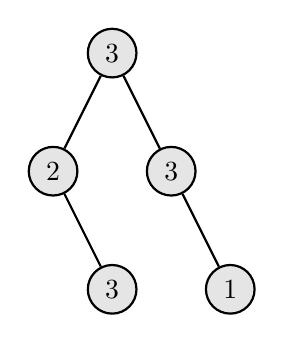
\begin{tikzpicture}
[every node/.style={draw, circle, fill=gray!20!, minimum size=5mm},
%level 1/.style={sibling distance=25mm},
%level 2/.style={sibling distance=15mm},
thick]
\node{3}
child{node{2} child[missing] child{node{3}}}
child{node{3} child[missing] child{node{1}}};
\end{tikzpicture}
\end{figure}

\textbf{Output}: 7
 
\textbf{Explanation}: Maximum amount of money the thief can rob is $3 + 3 + 1 = 7$.
\end{flushleft}

\paragraph{Example 2:}
\begin{flushleft}


\textbf{Input}: \fcj{[3,4,5,1,3,null,1]}

\begin{figure}[H]
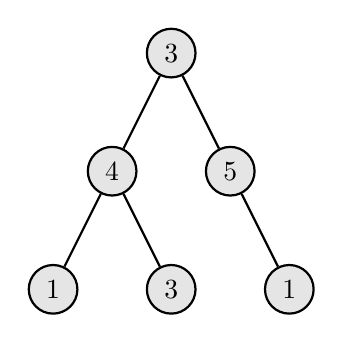
\begin{tikzpicture}
[every node/.style={draw, circle, fill=gray!20!, minimum size=5mm},
%level 1/.style={sibling distance=25mm},
%level 2/.style={sibling distance=15mm},
thick]
\node{3}
child{node{4} child{node{1}} child{node{3}}}
child{node{5} child[missing] child{node{1}}};
\end{tikzpicture}
\end{figure}

\textbf{Output}: 9

\textbf{Explanation}: Maximum amount of money the thief can rob is $4 + 5 = 9$.

\end{flushleft}

\setcounter{lstlisting}{0}
\begin{lstlisting}[style=customc, caption={DFS}]
int rob( TreeNode* root )
{
    unordered_map<TreeNode*, int> memo;
    return dfs( root, memo );
}
int dfs( TreeNode* t, unordered_map<TreeNode*, int>& memo )
{
    if( !t )
    {
        return 0;
    }
    auto it = memo.find( t );
    if( it != memo.end() )
    {
        return it->second;
    }
    //first find the value of rob t
    int val = 0;
    if( t->left )
    {
        val += dfs( t->left->left, m ) + dfs( t->left->right, m );
    }

    if( t->right )
    {
        val += dfs( t->right->left, m ) + dfs( t->right->right, m );
    }
    //now find the value of not robbing t
    int rob_without_t = dfs( t->left, m ) + dfs( t->right, m );
    val = ( max )( val + root->val, rob_without_t );
    memo.emplace( t, val );
    return val;
}
\end{lstlisting}